% !TeX root = ../main.tex
%
\chapter{State Estimation}
There are three measurable states in the twin pendulum system, the pendulum angles, $\theta_1$ and $\theta_2$, and the position of the cart, $x$. The renaming three states, the pendulum velocities, $\dot{\theta}_1$ and $\dot{\theta}_2$, and the cart velocity, $\dot{x}$, must be estimated. In this chapter a Kalman filter is designed based on \cite{haugen2015kompendium, rhudy2017kalman}.\\
The pendulum angles are measured with a resolution of $\Delta_\theta =\ $\SI{\pi e-3} rad/tic and the cart position with a resolution of $\Delta_x =\ $\SI{0.088e-3} m/tic. This causes the quantization problem illustrated for $\theta_1$ in \autoref{fig:quantizationProblem}. This is less of an issue for $x$ since its measurement resolution is two orders of magnitude higher than that of the angles.
%
\begin{figure}[H]
  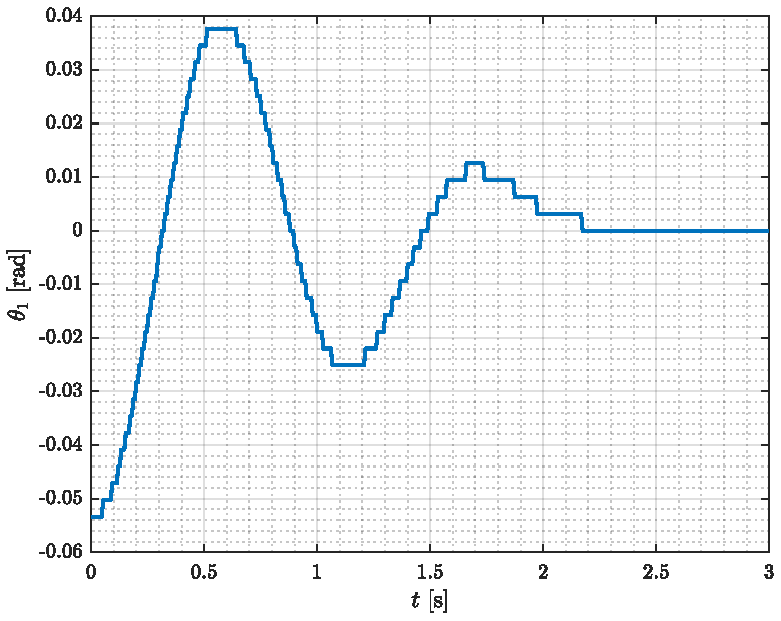
\includegraphics[width=.7\textwidth]{figures/quantizationProblem}
  \caption{Angle measurement of the first pendulum shows how the quantization is more significant than any potential underlying noise.}
  \label{fig:quantizationProblem}
\end{figure}
%
To estimate the three unmeasured states and solve the quantization problem a Kalman filter is designed. In the design process it is useful to have a simulation exhibiting the same issues as the real system. To that end a simple quantization model, \cite[35]{dutoit2010applied}, is proposed,
\begin{align}
x_q = \Delta \left\lfloor\ \frac{x}{\Delta} + \frac{1}{2}\ \right\rfloor \ \ \ ,   \label{eq:quantizationModel}
\end{align}
where $x_q$ is the quantized state, $x$ is the un-quantized simulated state and $\Delta$ is the measurement resolution of said state. To see if the model behaves like the real measurements, the original signal from \autoref{fig:quantizationProblem} is smoothed and then quantized using \autoref{eq:quantizationModel}. The result is seen in \autoref{fig:quantizationProblemModel} where the modeled quantization of the smoothed signal approaches the original measured signal.
%
\begin{figure}[H]
  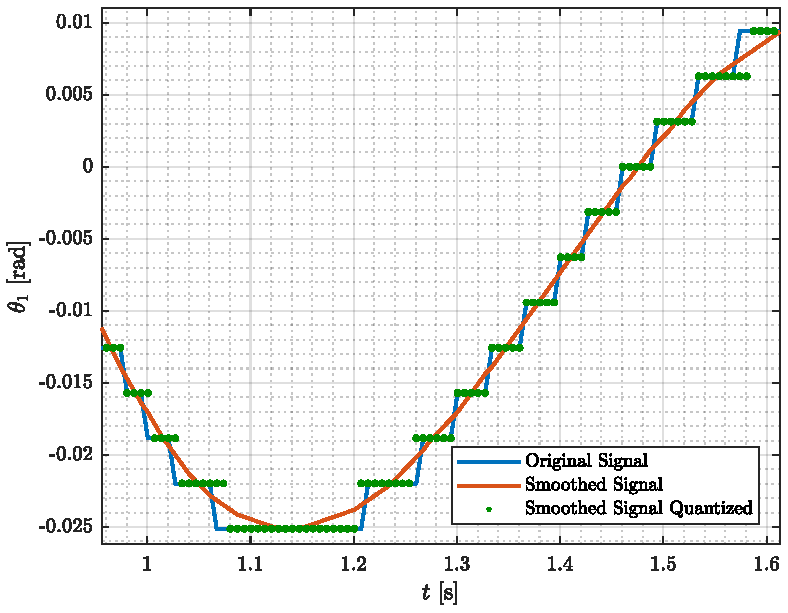
\includegraphics[width=.7\textwidth]{figures/quantizationProblemModel}
  \caption{The original measured signal (blue) is smoothed (red) and the smoothed signal is then quantized (green) using the model from \autoref{eq:quantizationModel}. This is used as a way to simulate measurements in the Kalman filter design process.}
  \label{fig:quantizationProblemModel}
\end{figure}
%
In this manner it is possible to simulate the system obtaining true values for all six states along with a quantized version for the Kalman filter.

The Kalman filter is designed using the following discrete linear model,
\begin{alignat}{3}
\vec{x}_{k} &= \vec{F} \vec{x}_{k-1} + \vec{G} u_{k-1} + \vec{w}_{k-1}  \ \ , &&\ \ \ \ \vec{w} \sim \mathcal{N}(0,\,\vec{Q})\,   \\
\vec{y}_k   &= \vec{H} \vec{x}_k + \vec{v}_k                              \ \ , &&\ \ \ \ \vec{v} \sim \mathcal{N}(0,\,\vec{R})\,  \ \ \ , 
  \label{eq:discreteModelForKF}
\end{alignat}
where,
\begin{table}[H]
  \vspace{-12pt}
  \begin{tabular}{l l l l}
    %-------------------------------------------------------------------------------------------------
      $\vec{x}$ is the states       &&& $\vec{F}$ is the system matrix                              \\
    %-------------------------------------------------------------------------------------------------
      $u$       is the input        &&& $\vec{G}$ is the input matrix                               \\
    %-------------------------------------------------------------------------------------------------
      $\vec{y}$ is the measurements &&& $\vec{H}$ is the output matrix                              \\
    %-------------------------------------------------------------------------------------------------
    \multicolumn{4}{l}
    {
      $\vec{w}$ is the process noise drawn from a normal distribution with covariance $\vec{Q}$
    }                                                                                               \\
    %-------------------------------------------------------------------------------------------------
    \multicolumn{4}{l}
    {
      $\vec{v}$ is the measurement noise drawn from a normal distribution with covariance $\vec{R}$\ .
    }                                                                                               \\
    %-------------------------------------------------------------------------------------------------
  \end{tabular}
  \vspace{-12pt}
\end{table}
%
In the following the Kalman filter algorithm is presented in three steps.
%
\subsubsection{Initialization}
The previous predicted state vector, $\hat{\vec{x}}_{k-1}$, is initialized to the current measurements, $y_k$,
%
\begin{align}
\hat{\vec{x}}_{k-1} &= y_k \ \ \ ,   \label{eq:xInit}
\end{align}
%
and the previous state error covariance $\vec{P}_{k-1}$ is initialized to some initial guess $\vec{P}_0$ here set to the identity matrix,
\begin{align}
\vec{P}_{k-1} &= \vec{P}_0  \ \ \ . \label{eq:initP}
\end{align}
%
When the Kalman filter is running $\vec{P}$ will converge to some steady state values which is then used as $\vec{P}_0$ in the implementation for faster convergence.

\subsubsection{Prediction}
A prediction of the states is calculated using the discrete system model,
\begin{align}
\hat{\vec{x}}_{k|k-1} &= \vec{F} \hat{\vec{x}}_{k-1} + \vec{G} u_{k-1} \ \ \ , \label{eq:predictedState}
\end{align}
where $\hat{\vec{x}}_{k|k-1}$ is the predicted states at time k using previous estimate and input. Note that $k|k-1$ reads ``$k$ given $k-1$''. Similarly a prediction of the state error covariance matrix is computed,
%
\begin{align}
\vec{P}_{k|k-1} &= \vec{F} \vec{P}_{k-1} \vec{F}^\mathrm{T} + \vec{Q}  \ \ \ , \label{eq:predictedStateErrorCovariance}
\end{align}
using the previous state error covariance matrix, $\vec{P}_{k-1}$, with state dynamics, $\vec{F}$, and the process noise covariance, $\vec{Q}$.
%
\subsubsection{Update}
The predicted state error covariance matrix, $\vec{P}_{k|k-1}$, is then used along with the output matrix, $\vec{H}$, and the measurement noise error covariance, $\vec{R}$, to compute the Kalman gain,
\begin{align}
\vec{K}_k &= \vec{P}_{k|k-1} \vec{H}^\mathrm{T} ( \vec{H} \vec{P}_{k|k-1} \vec{H}^\mathrm{T} + \vec{R} )^{-1}  \ \ \ . \label{eq:kalmanGain}
\end{align}
Finally the estimated states are updated using the previous estimated states, $\hat{\vec{x}}_{k-1}$, the Kalman gain, $ \vec{K}_k$, and the difference between measured output, $y_k$, and predicted output,
\begin{align}
\hat{\vec{x}}_k &= \hat{\vec{x}}_{k-1} + \vec{K}_k ( y_k - \vec{H} \hat{\vec{x}}_{k-1} ) \ \ \ , \label{eq:estimatedState}
\end{align}
where $\vec{H} \hat{\vec{x}}_{k-1} = \hat{\vec{y}}_{k-1}$ is the predicted output. The state error covariance matrix is also updated,
%
\begin{align}
\vec{P}_k &= ( \vec{I} - \vec{K}_k \vec{H} ) \vec{P}_{k|k-1} \ \ \ , \label{eq:stateErrorCovariance}
\end{align}
where $\vec{I}$ is the identity matrix.

The measurement noise covariance is tuned such that the quantization problem is solved without causing divergence from the trend of the data, see \autoref{fig:theta1_KFsim},
\begin{align}
\vec{R} &= diag( 100,\ 100,\ 10 )  \ \ \ .
\end{align}
%
\begin{figure}[H]
  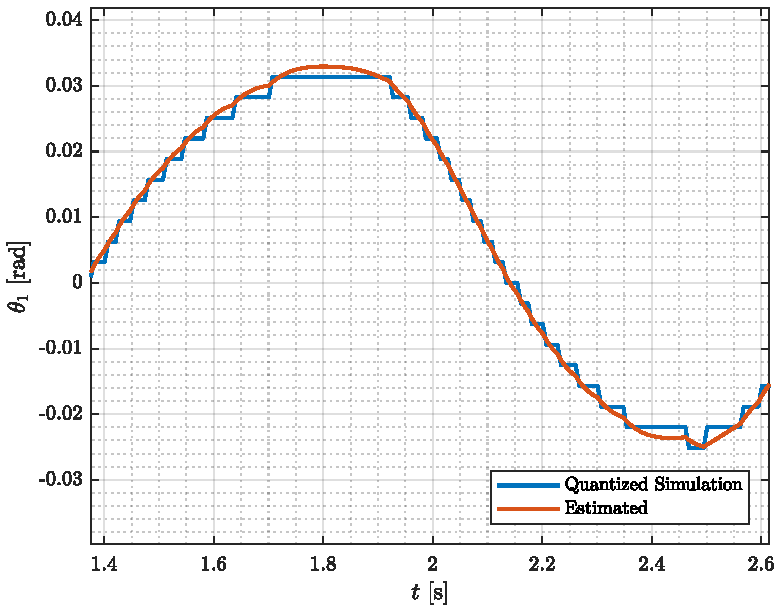
\includegraphics[width=.7\textwidth]{figures/theta1_KFsim}
  \caption{The Kalman filter successfully overcomes the quantization problem in simulation. A similar result is obtained for $\theta_2$.}
  \label{fig:theta1_KFsim}
\end{figure}
%
The process noise covariance matrix is tuned to get as true estimations of the derivatives as possible while maintaining low noise levels, see simulation in \autoref{fig:theta1Dot_KFsim},
\begin{align}
\vec{Q} &= diag( 1,\ 1,\ 1,\ 100,\ 100,\ 10 )  \ \ \ ,
\end{align}
%
\begin{figure}[H]
  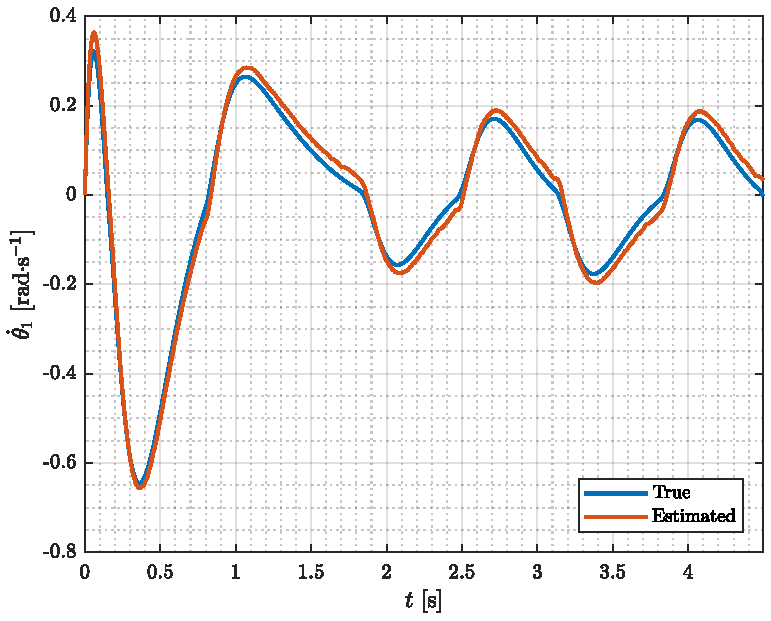
\includegraphics[width=.7\textwidth]{figures/theta1Dot_KFsim}
  \caption{Simulation of LQR controller used for tuning the Kalman filter to get a good estimation of the state derivatives. A similar result is obtained for $\dot{\theta}_2$.}
  \label{fig:theta1Dot_KFsim}
\end{figure}
%
Since the quantization problem is less significant for the position measurements compared to the angle measurements, the filter obtains near perfect results in simulation, see \autoref{fig:x_KFsim} and \ref{fig:xDot_KFsim}.
%
\begin{figure}[H]
  \hspace{-10pt}
  \captionbox
  {
    The quantization of $x$ is so insignificant that it does not show on the plot.
    \label{fig:x_KFsim}
  }
  {
    \hspace{-1cm}
    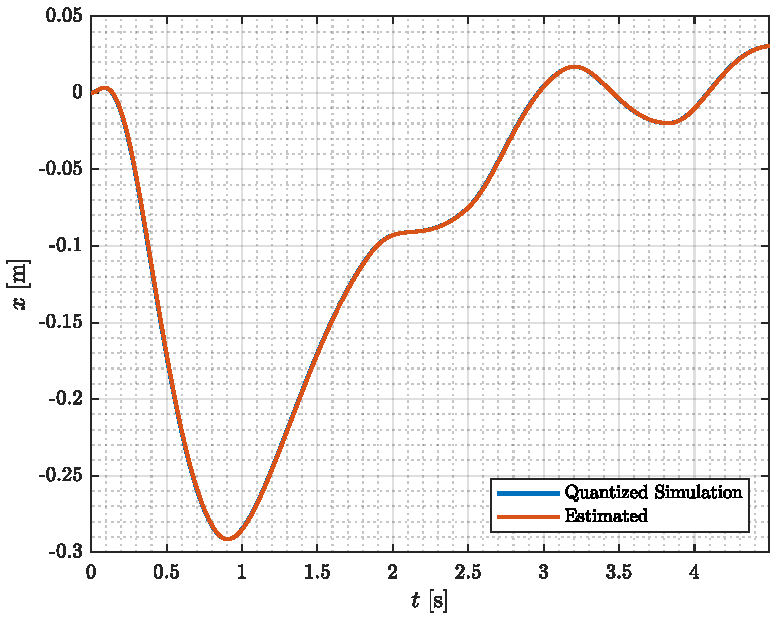
\includegraphics[width=.5\textwidth]{figures/x_KFsim}
  }
  \hspace{20pt}
  \captionbox 
  {
    Given the good position measurements, the Kalman filter successfully estimates the cart velocity.
    \label{fig:xDot_KFsim}
  }
  {
    \hspace{-1cm}
    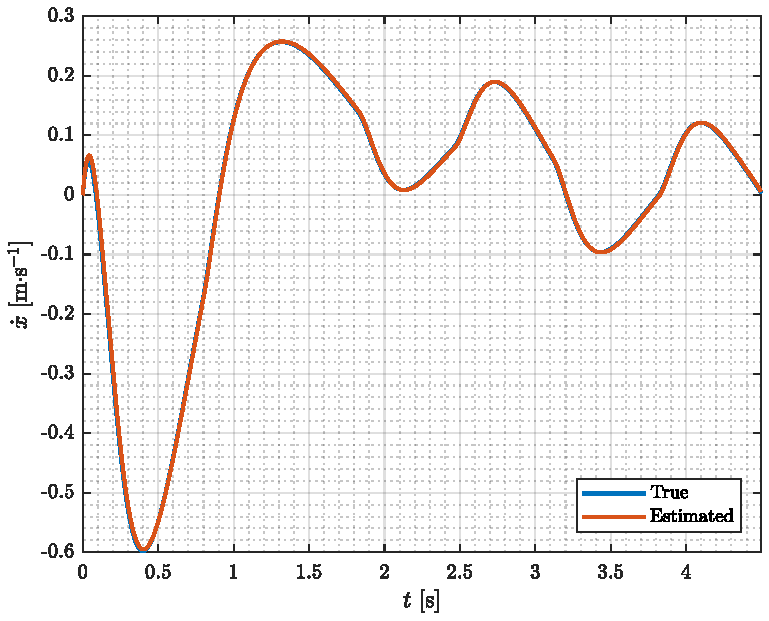
\includegraphics[width=.5\textwidth]{figures/xDot_KFsim}
  }  
\end{figure}
%
%other available plots
% theta2_KFsim
% theta2Dot_KFsim
%
%
%
%
%
%-------plots-----------
%
%  implemented Kalman filter  (maybe have it in results)
%
%
%
This concludes state estimation for the twin pendulum system. With all parameters estimated and the Kalman filter designed for state estimation any remaining comments on implementation are addressed when presenting the results in the next chapter.